\subsection{Capas de la arquitectura}

Las ocho capas separan la interacción con las personas, las reglas de negocio y la persistencia. Seguridad y observabilidad atraviesan el conjunto. La vista general permite ubicar cada responsabilidad antes de revisar sus componentes; el inventario trazable se reúne en el Anexo 4.1-N.

Presentación reúne las superficies de trabajo; borde protege su entrada; puerta de enlace valida solicitudes; negocio decide por módulo; integración intercambia contratos; acceso a datos persiste por propietario. Seguridad y observabilidad atraviesan esas seis responsabilidades.

{\footnotesize Fuente: elaboración propia de LafroX a partir de Bases Técnicas Transversales, numeral 2.1.\par}

Las capas 7 y 8 atraviesan las demás; no duplican reglas de negocio.

La arquitectura se presenta primero mediante su vista general completa (Figura~\ref{fig:arql-general-completa}) y después mediante una síntesis de sus ocho capas (Figura~\ref{fig:arql-1}). Ambas vistas se complementan para relacionar las funciones de negocio con los componentes que las sostienen.

\clearpage
\begin{center}
  \includegraphics[width=\linewidth,height=0.83\textheight,keepaspectratio]{Diagramas/arquitectura_logica_actual/cambios laravel/ARQL-01_Vision_general.png}
  \captionof{figure}{Vista general completa de la arquitectura lógica}
  \label{fig:arql-general-completa}
\end{center}
{\footnotesize Fuente: diagrama general aportado por Tomás Pérez; LafroX.\par}

La vista general muestra cómo cada actor accede a la solución desde su aplicación, portal o consola y se relaciona con los módulos M1--M12. Se lee desde las personas hacia las reglas de negocio, las integraciones y los datos, distinguiendo los componentes de nube y los del sitio. Las conexiones representan intercambios sujetos a autorización, no acceso directo a las bases de datos. Seguridad y observabilidad acompañan todo el recorrido; sus controles y las condiciones de operación sin conexión se desarrollan en los apartados siguientes.

\clearpage
\begin{center}
  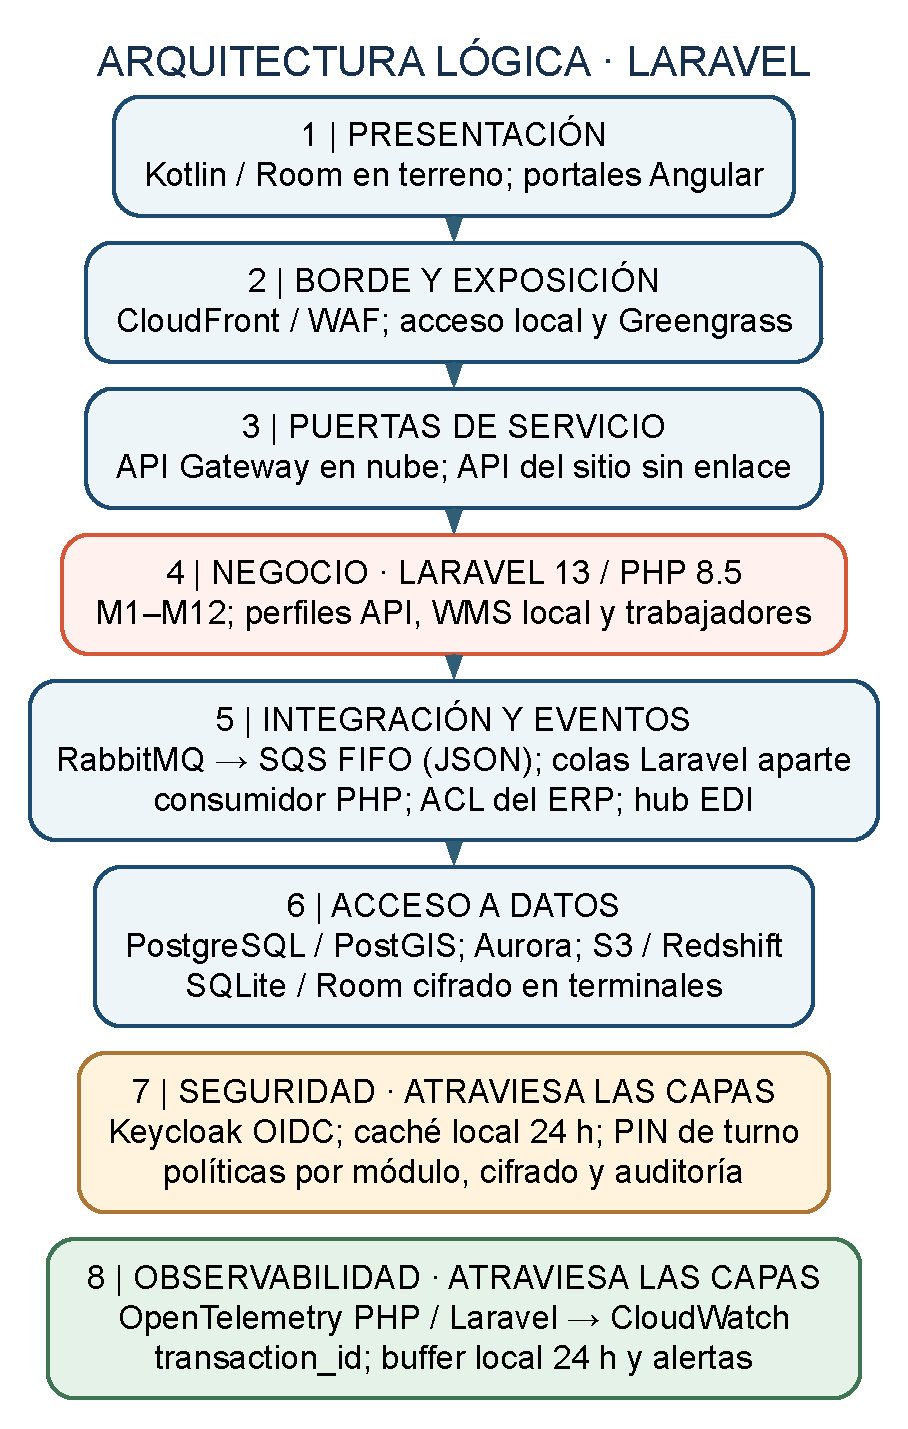
\includegraphics[width=0.98\linewidth,height=0.65\textheight,keepaspectratio]{Diagramas/arquitectura_logica_actual/ARQL-19_Vista_general_legible.pdf}
  \captionof{figure}{Vista resumida de las ocho capas lógicas}
  \label{fig:arql-1}
\end{center}

{\footnotesize Fuente: elaboración propia de LafroX.\par}

La vista resumida destaca la responsabilidad de cada capa: presentación captura y muestra información; borde protege la entrada; las puertas de servicio validan las solicitudes; el negocio aplica las reglas en Laravel; integración conserva y distribuye eventos; y acceso a datos administra la persistencia. Seguridad y observabilidad son transversales, no pasos finales del procesamiento. La puerta local permite que la bodega siga operando sin WAN, mientras las colas conservan el trabajo pendiente para reconciliarlo al recuperar la conexión.

\clearpage
\subsubsection{Capa de presentación}

La Figura~\ref{fig:arql-capa-1} presenta las responsabilidades de esta capa.

\begin{center}
  \begin{minipage}{\linewidth}\centering
  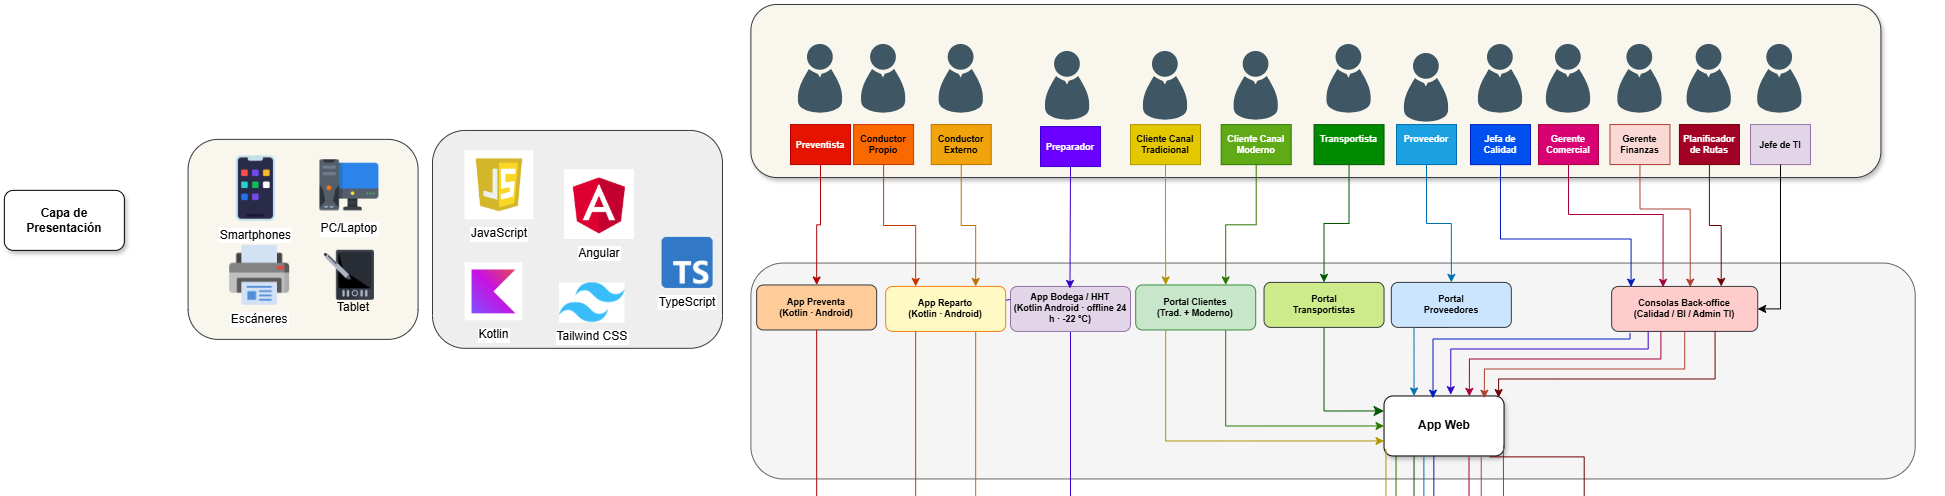
\includegraphics[width=0.98\linewidth,height=0.60\textheight,keepaspectratio]{Diagramas/arquitectura_logica_actual/capas_recortes/ARQL-21_Recorte_Presentacion.png}
  \captionof{figure}{Presentación: aplicaciones y superficies de trabajo}
  \label{fig:arql-capa-1}
  \par\smallskip
  {\raggedright\footnotesize Fuente: recorte por capa del diagrama general aportado por Tomás Pérez; LafroX.\par}
  \end{minipage}
\end{center}

Las aplicaciones móviles conservan las capturas pendientes; los portales y consolas consultan sus dominios mediante APIs autorizadas. El dispositivo y la pantalla no sustituyen la identidad ni los permisos de la persona.


La capa de presentación reúne las herramientas que utiliza cada persona para trabajar: aplicaciones móviles que pueden operar sin conexión y portales web servidos desde la nube. Preventistas, conductores y preparadores capturan hechos operativos; clientes, transportistas y proveedores consultan únicamente sus datos autorizados; Calidad, gerencias, planificación y TI toman decisiones desde consolas especializadas. Los permisos se asignan mediante una matriz de roles y atributos: un perfil de interacción no implica por sí solo acceso a todas las funciones del módulo.

Las aplicaciones de campo (preventa y reparto) se construyen en Kotlin nativo para Android, decisión alineada con el ecosistema del parque de dispositivos Zebra (EC55, TC58e, MC9400) desplegado en los centros de distribución y con las condiciones de operación del terreno. La app de preventa mantiene una foto local de datos de lectura (stock, precios, crédito, promociones) y captura local de eventos (pedidos, identificadores únicos UUID); la app de reparto gestiona la entrega, la prueba de entrega digital (POD con firma, código QR y fotografía), la cobranza en ruta y el control de envases retornables. Ambas aplicaciones operan con datos locales cifrados y sincronizan de forma idempotente por medio del API Gateway cuando se recupera la conectividad.

Los terminales de bodega (HHT con escáner GS1) descargan las misiones de preparación al inicio del turno y registran su ejecución localmente, incluso en cámaras a -22 °C sin señal. La autonomía mínima de 24 horas comprende el servicio de bodega completo: registro de operaciones, conservación de datos, cambios de turno y control de acceso.

Los portales web, implementados en Angular con Tailwind CSS, permiten a clientes consultar pedidos y documentos, a transportistas revisar rutas y a proveedores consultar órdenes y recepciones. El catálogo público admite consulta sin autenticación; las funciones privadas requieren identidad OIDC mediante Keycloak y permisos por rol. El acceso administrativo exige MFA y una ruta autorizada, definida físicamente en 4.2.

Las consolas de rutas, calidad, BI y administración TI acceden a sus dominios mediante APIs autorizadas. Ningún navegador se conecta directamente a las bases de datos. Esta separación permite aplicar las mismas reglas de acceso y auditoría con independencia de la pantalla utilizada.

\subsubsection{Capa de borde y exposición (Capa 2)}

La Figura~\ref{fig:arql-capa-2} presenta las responsabilidades de esta capa.

\begin{center}
  \begin{minipage}{\linewidth}\centering
  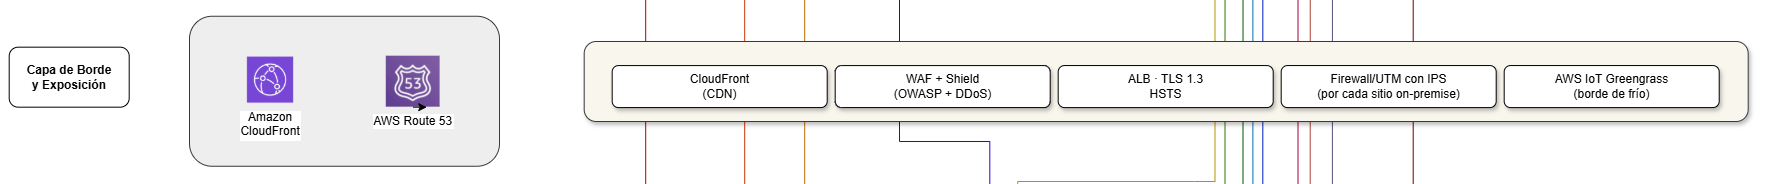
\includegraphics[width=0.98\linewidth,height=0.60\textheight,keepaspectratio]{Diagramas/arquitectura_logica_actual/capas_recortes/ARQL-22_Recorte_Borde.png}
  \captionof{figure}{Borde: entradas públicas, privadas y locales}
  \label{fig:arql-capa-2}
  \par\smallskip
  {\raggedright\footnotesize Fuente: recorte por capa del diagrama general aportado por Tomás Pérez; LafroX.\par}
  \end{minipage}
\end{center}

La entrada pública protege las APIs y rechaza el acceso directo a su origen. El acceso local sostiene la bodega sin WAN; Greengrass procesa los sensores de cámara, mientras AS2 conserva una superficie B2B distinta.


La capa de borde delimita la entrada pública y la entrada de dispositivos de terreno y bodega, donde la conectividad es intermitente. Define las siguientes responsabilidades; su despliegue se especifica en 4.2:

\begin{itemize}
  \item \textbf{CDN (Amazon CloudFront).} Entrada pública de portales externos y APIs de negocio: distribuye contenido estático y encamina las rutas \texttt{/v1} y \texttt{/sync/v1} al API Gateway. El acceso directo al origen de esas APIs debe rechazarse y probarse. Las consolas internas usan acceso privado verificado; el transporte AS2 tiene una superficie separada, restringida a contrapartes registradas.
  \item \textbf{WAF gestionado (AWS WAF + Shield).} Filtrado de tráfico con reglas OWASP Top 10 y reglas personalizadas por API; protección contra denegación de servicio en capas 3, 4 y 7.
  \item \textbf{Balanceador de carga (ALB).} Distribuye hacia los servicios privados el tráfico que API Gateway entrega mediante su integración privada. El flujo de acceso público es cliente $\rightarrow$ CloudFront/WAF $\rightarrow$ API Gateway $\rightarrow$ integración privada/ALB $\rightarrow$ servicio.
  \item \textbf{Acceso local y continuidad.} Los servicios del sitio aplican control de acceso propio y preservan la operación crítica aun cuando todos los enlaces externos estén indisponibles. Los CD usan fibra y LTE; los cross-docking usan Starlink y LTE de dos proveedores, con conmutación automática en menos de 30 segundos (ADR-02).
  \item \textbf{AWS IoT Greengrass.} Corre solo en dos gateways IoT industriales (Moxa UC-8200 o equivalente), uno en el CD Talca y otro en el CD Concepción. Leen los sensores de cámara por Modbus, bloquean el despacho ante una excursión térmica en menos de 5 segundos y conservan 24 horas de datos sin enlace. No se instala en camiones: la posición de la flota llega por la API del tercero (INT-15). Los termógrafos registran toda la ruta en su memoria interna, avisan por BLE al terminal del conductor aun sin señal y este reenvía el aviso a la nube al recuperar cobertura; al volver el camión, el terminal descarga y envía el registro completo.
\end{itemize}

\subsubsection{Capa de puerta de enlace de servicios (Capa 3)}

La Figura~\ref{fig:arql-capa-3} presenta las responsabilidades de esta capa.

\begin{center}
  \begin{minipage}{\linewidth}\centering
  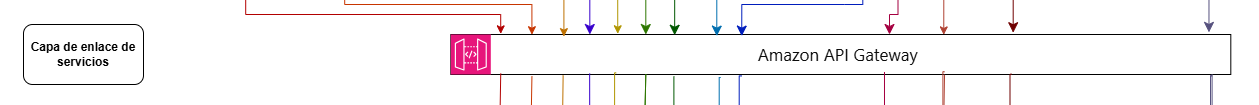
\includegraphics[width=0.98\linewidth,height=0.60\textheight,keepaspectratio]{Diagramas/arquitectura_logica_actual/capas_recortes/ARQL-23_Recorte_Puertas.png}
  \captionof{figure}{Puertas de servicio: recorrido central y local}
  \label{fig:arql-capa-3}
  \par\smallskip
  {\raggedright\footnotesize Fuente: recorte por capa del diagrama general aportado por Tomás Pérez; LafroX.\par}
  \end{minipage}
\end{center}

El recorrido central valida la identidad y entrega solicitudes a servicios privados. La puerta local atiende al HHT dentro del sitio, sin invocar el Gateway remoto durante un corte; ambos recorridos conservan validación, idempotencia y auditoría.


Amazon API Gateway concentra la publicación de servicios detrás de la entrada pública de CloudFront. El diseño requiere validar la identidad emitida por Keycloak, controlar esquema, cuotas y tasa de solicitudes, y propagar un \texttt{transaction\_id}. Se selecciona REST API con authorizer REQUEST que verifica firma, emisor, audiencia, expiración y alcance del JWT de Keycloak. Las operaciones sensibles no reutilizan autorizaciones almacenadas; el módulo verifica además recurso y revocación conocida. La integración privada usa VPC Link V2 hacia ALB; la validación básica de Gateway se complementa con el esquema completo en Laravel (AWS, s.~f.-a, s.~f.-b, s.~f.-c; Anexo 4.1-O, ADR-13). El recorrido físico y el bloqueo efectivo del acceso directo al origen se deben comprobar en 4.2.

La capa publica dos conjuntos de APIs: las de negocio (\texttt{/v1}) y las de sincronización offline (\texttt{/sync/v1}). El Gateway aplica los controles de entrada y enruta las solicitudes. El servicio de negocio valida el contenido y garantiza la idempotencia de cada escritura mediante su UUID, una ventana de deduplicación documentada y el registro persistente del resultado (RT-02.06).

El ingreso por API Gateway corresponde a los servicios en nube. Durante una interrupción del enlace, la bodega utiliza los servicios de su sitio sin depender del Gateway remoto. Los terminales sin cobertura conservan sus eventos y los entregan al servicio local cuando recuperan comunicación; la reconciliación con la nube ocurre al restablecerse el enlace externo. Los contratos y las reglas de validación se mantienen en ambos recorridos.

La bodega dispone además de una puerta de API \emph{local} como función del motor WMS A-01, en VM-01, VM-C01 y E-01, acotada a la red del sitio y a M1, M2, M5 y la función local de bloqueo de M9. Los 120 terminales no llaman a Amazon API Gateway durante un corte: el verificador local valida la autorización de turno y esta función aplica esquema, límites de tasa, tamaño de carga, UUID y registro de auditoría antes de entregar una orden al módulo correspondiente. Este control no publica una segunda entrada en internet ni emite identidades nuevas. La Figura~\ref{fig:arql-17} separa los dos recorridos y muestra cómo se conserva el trabajo hasta la reconexión.

\begin{center}
  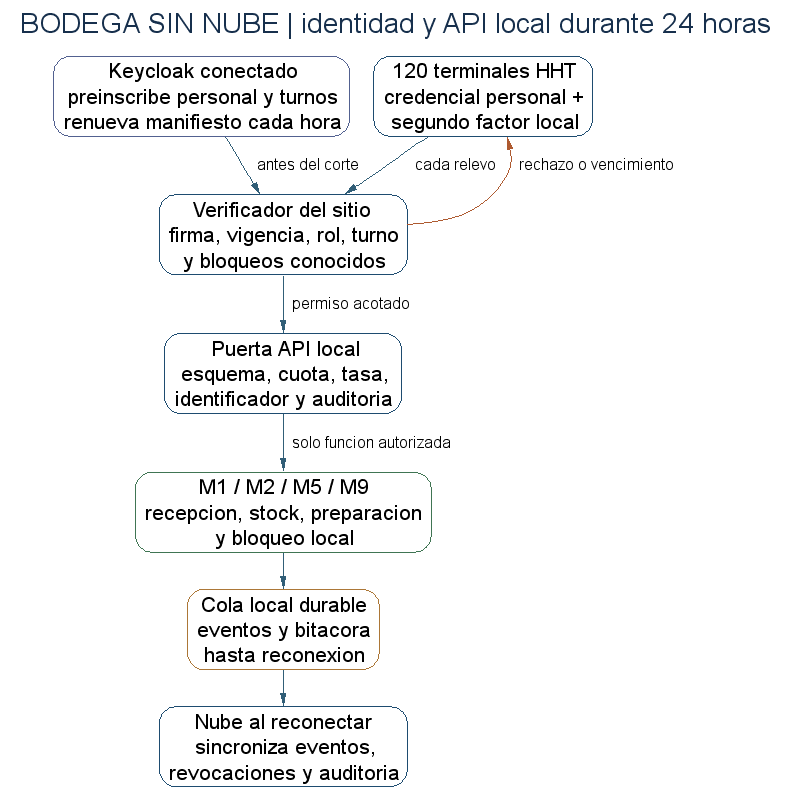
\includegraphics[width=0.96\linewidth,height=0.72\textheight,keepaspectratio]{Diagramas/arquitectura_logica_actual/ARQL-17_Acceso_local_24h.png}
  \captionof{figure}{Identidad y puerta de API local durante un corte de 24 horas}
  \label{fig:arql-17}
\end{center}

{\footnotesize Fuente: elaboración propia de LafroX.\par}

El manifiesto de turno firmado por Keycloak llega antes del corte; en cada relevo el verificador local, alojado junto a la caché, valida el manifiesto y un segundo factor local: el PIN personal sobre el terminal enrolado por MDM. El permiso queda limitado a funciones de bodega, mientras los eventos y la bitácora se envían después con su identificador original. La prueba debe iniciar el corte antes de dos relevos sucesivos y medir vencimiento, denegación, reintentos y recuperación; la caché de identidad de 24 horas no emite sesiones y el relevo lo habilita el verificador local.

\subsubsection{Capa de lógica de negocio (Capa 4)}

La Figura~\ref{fig:arql-capa-4} presenta las responsabilidades de esta capa.

\begin{center}
  \begin{minipage}{\linewidth}\centering
  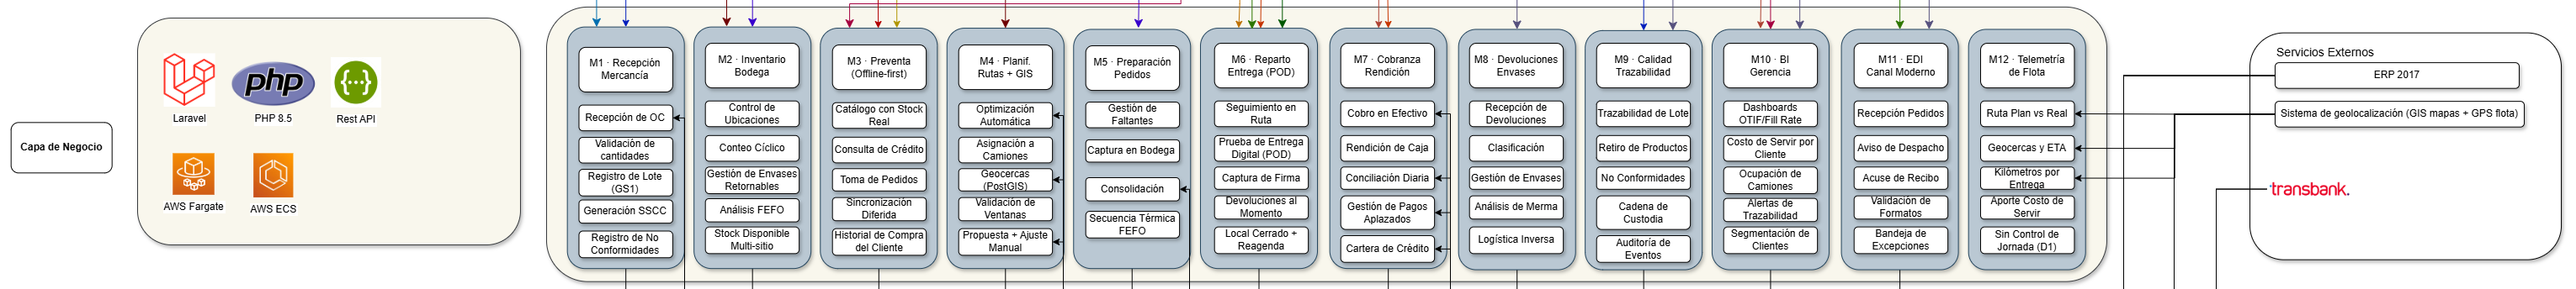
\includegraphics[width=0.98\linewidth,height=0.60\textheight,keepaspectratio]{Diagramas/arquitectura_logica_actual/capas_recortes/ARQL-24_Recorte_Negocio.png}
  \captionof{figure}{Negocio: monolito modular Laravel y sus doce módulos}
  \label{fig:arql-capa-4}
  \par\smallskip
  {\raggedright\footnotesize Fuente: recorte por capa del diagrama general aportado por Tomás Pérez; LafroX.\par}
  \end{minipage}
\end{center}

El recorte reúne los doce módulos de negocio y sus funciones principales, junto con las tecnologías del backend y los sistemas externos con los que se relacionan. Los límites e intercambios de cada contexto se desarrollan en los apartados siguientes.


La capa de servicios de negocio reúne M1--M12 en un monolito modular Laravel. Cada contexto separa \texttt{Domain}, \texttt{Application}, \texttt{Infrastructure} y \texttt{Http} bajo un espacio de nombres PSR-4. Los controladores reciben y validan solicitudes; los servicios de aplicación coordinan casos de uso; el dominio decide reservas, bloqueos y rendiciones; los adaptadores traducen persistencia e integraciones. Los módulos se llaman mediante interfaces públicas o eventos versionados: no acceden a las tablas privadas de otro contexto ni importan sus modelos de persistencia. Los proveedores de servicios registran esas interfaces en el contenedor y una prueba de dependencias impide invertir las fronteras. Así, compartir proceso no confunde la propiedad de cada decisión (RT-02.05).

La misma versión del artefacto Laravel ejecuta perfiles separados: API central, WMS local limitado a M1/M2/M5 y bloqueo M9, consumidores de SQS, adaptador AMQP y reglas comerciales EDI de M11. El transporte OpenAS2 es un componente independiente: verifica certificados, firma, cifrado y acuses MDN antes de entregar el mensaje a M11; no ejecuta reglas comerciales ni escribe en el ERP. Cada perfil dispone de cola, concurrencia, permisos y métricas propios. El planificador de tareas tiene una sola autoridad por ambiente. Esta separación permite escalar y reiniciar sincronización, EDI y telemetría sin multiplicar el monolito completo (RT-02.02).

Los módulos evitan estado durable en memoria y pueden crecer por réplicas o por trabajadores independientes, según la demanda. Los umbrales, límites de capacidad, emplazamiento y costos se especifican en 4.2 y en la oferta económica.

\subsubsection{Capa de integración y eventos (Capa 5)}

La Figura~\ref{fig:arql-capa-5} presenta las responsabilidades de esta capa.

\begin{center}
  \begin{minipage}{\linewidth}\centering
  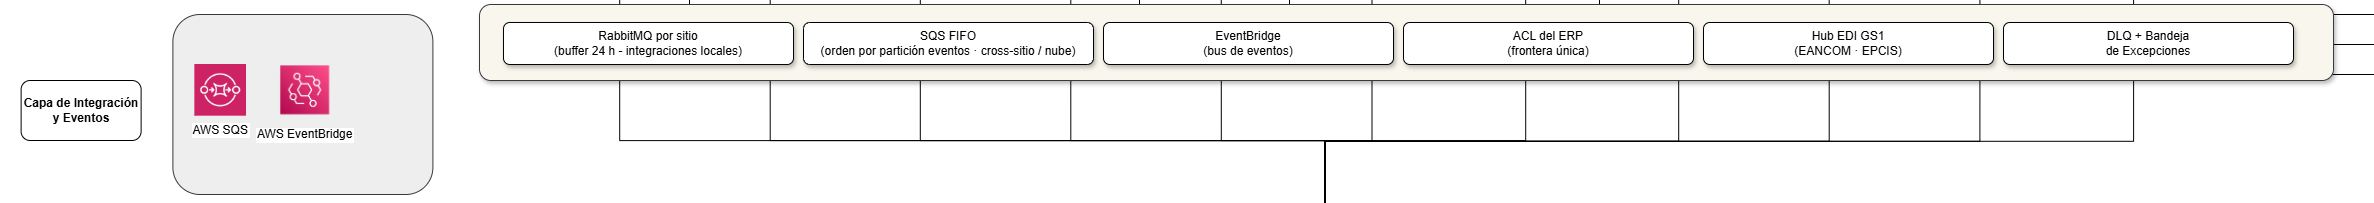
\includegraphics[width=0.98\linewidth,height=0.60\textheight,keepaspectratio]{Diagramas/arquitectura_logica_actual/capas_recortes/ARQL-25_Recorte_Integracion.png}
  \captionof{figure}{Integración: continuidad local y contratos con terceros}
  \label{fig:arql-capa-5}
  \par\smallskip
  {\raggedright\footnotesize Fuente: recorte por capa del diagrama general aportado por Tomás Pérez; LafroX.\par}
  \end{minipage}
\end{center}

El sitio conserva los eventos hasta confirmar su publicación y el consumidor confirma después de persistir. La ACL concentra el acceso al ERP, único emisor tributario; el hub EDI traduce contratos comerciales y las excepciones permanecen trazables.


La capa de integración conecta la nueva operación con sistemas que Puelche ya utiliza. Sus límites son especialmente importantes ante el ERP de 2017 sin interfaces documentadas y el WMS de 2013. También concentra el intercambio con cadenas del canal moderno, los servicios de pago, los mapas y la telemetría, de modo que un cambio externo no obligue a modificar cada módulo de negocio.

RabbitMQ conserva las colas de integración local. En nube, SQS FIFO ordena los mensajes de reconciliación dentro de cada grupo y SNS difunde eventos y alertas. Los avisos al cliente se entregan mediante SNS o la API del proveedor de notificaciones (INT-11). El orden no se presume global ni se atribuye a toda la cadena de eventos. Los consumidores aplican deduplicación, reintentos con espera creciente y una cola de mensajes fallidos (DLQ), con intervención trazable cuando el procesamiento no puede completarse (RT-02.07).

El shipper publica en la cola SQS FIFO de reconciliación un sobre JSON independiente de PHP con versión, identidad, clave de orden y carga. Un consumidor PHP dedicado lee ese sobre mediante el SDK de AWS, valida su esquema, invoca el caso de uso Laravel y reconoce el mensaje solo después de persistir el resultado. Los trabajos derivados propios de Laravel usan su conector SQS en colas distintas y declaran grupo y clave de deduplicación cuando requieren orden FIFO. Esta separación evita entregar mensajes externos al deserializador de trabajos del framework. RabbitMQ local se conecta mediante un adaptador AMQP probado con \texttt{php-amqplib}; el shipper confirma la publicación en SQS antes de reconocer el mensaje local. No se introduce Redis ni Horizon en los sitios, donde la continuidad depende de PostgreSQL y RabbitMQ.

Las APIs de la plataforma reciben solicitudes por la Capa 3. Los servicios de negocio invocan sus adaptadores de integración cuando necesitan consultar pagos o mapas, con tiempo máximo de espera explícito (RT-02.08). Los intercambios diferidos con ERP, EDI, telemetría y notificaciones utilizan colas y reintentos. La emisión tributaria se canaliza por el ERP mediante la ACL; no se crea un segundo emisor de documentos ante el SII.

El ERP de 2017 se conserva como única fuente de verdad tributaria y único emisor de DTE. La capa anticorrupción (ACL) traduce los contratos de la solución al formato del legado, sin reemplazarlo ni modificar su código. El flujo de rendición es: rendición aprobada $\rightarrow$ SQS $\rightarrow$ trabajador Laravel \texttt{erp-sync} $\rightarrow$ ACL $\rightarrow$ ERP. Ningún módulo, portal o cadena escribe directamente en el ERP. El trabajador usa una clave idempotente por operación y conserva folio, estado y acuse para seguir cada documento hasta su origen; reintentar un trabajo no solicita un segundo documento.

La integración con las cadenas del canal moderno se resuelve con un hub EDI centralizado en nube. Utiliza mensajes comerciales EANCOM y GS1 XML, y eventos EPCIS para trazabilidad. Cada cadena dispone de un conector configurable, una tabla de equivalencias GTIN (RF-12.03) y una bandeja de excepciones (RF-12.06). El hub transforma los mensajes al modelo canónico y entrega al ERP, exclusivamente mediante la ACL, la información necesaria para sus documentos, incluida la guía de despacho electrónica (GDE). AS2 es uno de los transportes del hub. El canal moderno debe quedar operativo a más tardar en enero de 2029.

\paragraph{Eventos canónicos del dominio.}
\label{subsubsec:eventos-canonicos}

Los eventos son el vocabulario del sistema. Se nombran en pasado, son inmutables y llevan \texttt{event\_id} (UUID), \texttt{occurred\_at}, \texttt{site\_id} y \texttt{transaction\_id}. El catálogo de eventos canónicos del dominio se presenta en el Anexo 4.1-A. Cada evento declara productor único, consumidores registrados, clave de partición y política de reintento, y su origen se traza a un requisito del caso o a una decisión del numeral 16.1.


Cada evento conserva productor único y clave de orden para evitar ambigüedad al reintentar.

Los esquemas AsyncAPI 2.6 versionados por evento se gobiernan desde el Catálogo de interfaces (\S~\ref{sec:catalogo-interfaces}); \texttt{transaction\_id} conserva la correlación entre los módulos consumidores.

\paragraph{Orquestación y coreografía.}
M3 coordina de manera síncrona la confirmación de un pedido y solicita a M2 una reserva: necesita una respuesta única y visible para el preventista. Cuando el pedido queda confirmado, publica \texttt{PedidoConfirmado}; M5, M4 y M10 reaccionan cada uno a ese hecho mediante su propio consumidor. Esa coreografía evita que M3 conozca el horario de preparación o el esquema analítico. La publicación se registra junto con el cambio de estado mediante una bandeja transaccional de salida (\textit{outbox}); el consumidor confirma su progreso solo después de persistir su resultado. Si falla un consumidor, la cola reintenta y termina en una bandeja de excepción, sin deshacer a ciegas el pedido ya confirmado.

El despacho tiene una coordinación distinta: M5 no libera la carga hasta recibir el resultado de M9 sobre el lote y la guía emitida por el ERP a través de la ACL. Una excursión térmica bloquea localmente la salida aun con el enlace caído; solo Calidad puede liberar el lote tras evaluación registrada. El conductor informa la incidencia y conserva la carga, pero no aprueba su liberación sanitaria. Las Figuras~\ref{fig:arql-15} y \ref{fig:arql-16} recorren el pedido con y sin conexión y hacen visible dónde cambia una captura pendiente a una operación confirmada.

\begin{center}
  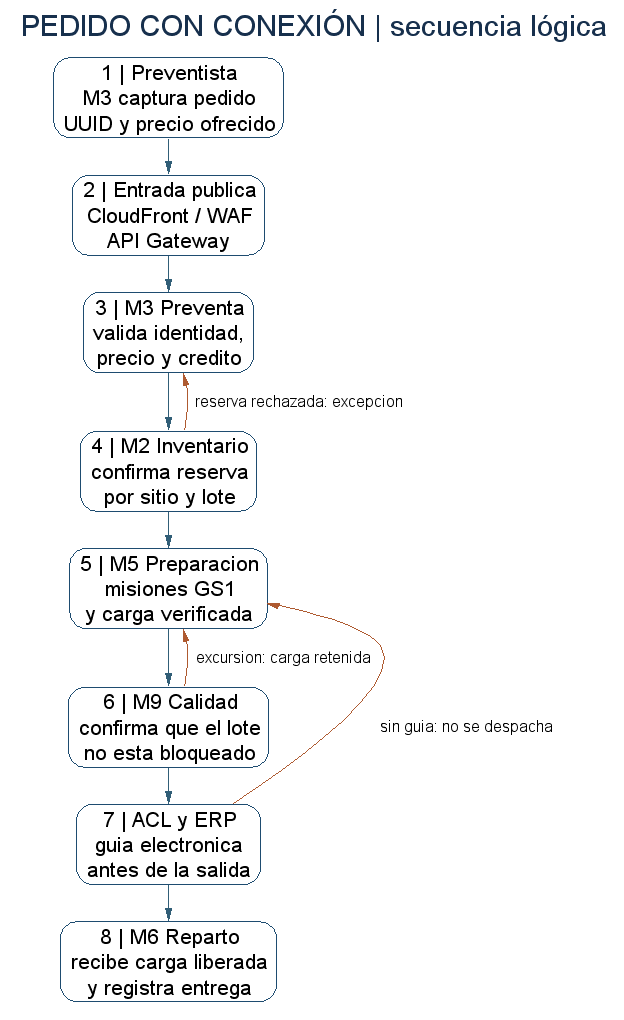
\includegraphics[width=0.96\linewidth,height=0.75\textheight,keepaspectratio]{Diagramas/arquitectura_logica_actual/ARQL-15_Pedido_con_conexion.png}
  \captionof{figure}{Secuencia lógica del pedido con conexión}
  \label{fig:arql-15}
\end{center}

{\footnotesize Fuente: elaboración propia de LafroX.\par}

Con conexión, M2 devuelve una reserva explícita y M5 no comienza a preparar un pedido rechazado. La carga preparada sigue retenida si M9 informa un bloqueo o si el ERP no devuelve la guía electrónica. El flujo dibuja esos dos retornos porque un pedido confirmado no autoriza por sí mismo la salida física.

\begin{center}
  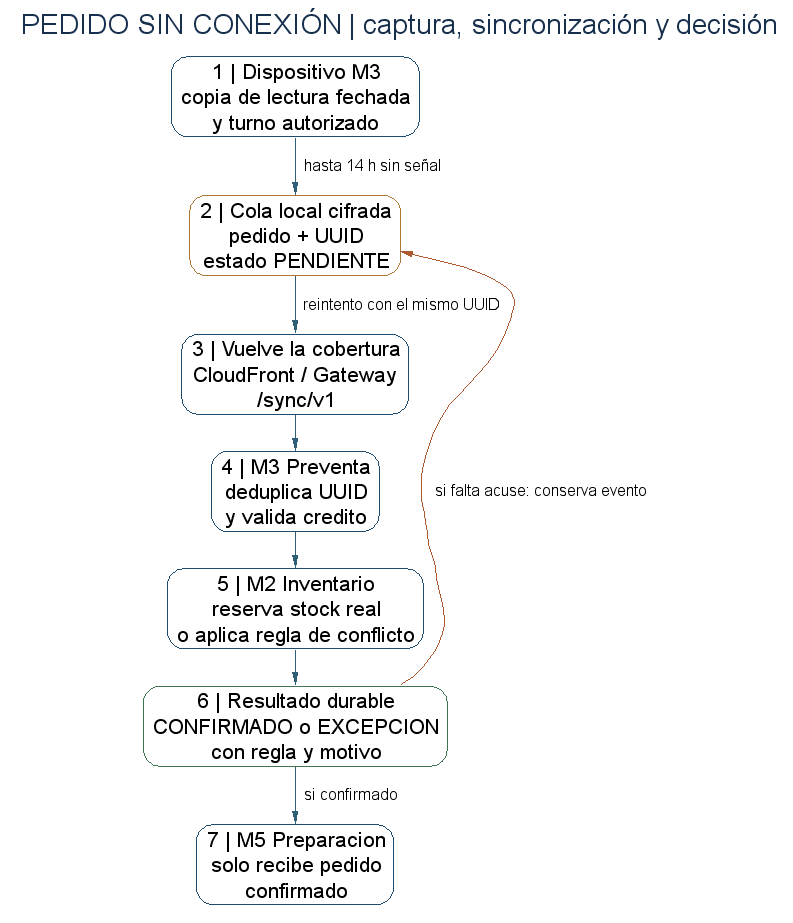
\includegraphics[width=0.96\linewidth,height=0.75\textheight,keepaspectratio]{Diagramas/arquitectura_logica_actual/ARQL-16_Pedido_sin_conexion.png}
  \captionof{figure}{Secuencia lógica del pedido capturado sin conexión}
  \label{fig:arql-16}
\end{center}

{\footnotesize Fuente: elaboración propia de LafroX.\par}

Sin conexión, la aplicación conserva la intención de compra, no una reserva firme. El mismo UUID viaja en todos los reintentos; M3 y M2 producen un resultado durable con la regla y la causal de excepción. Si se pierde el acuse de respuesta, el dispositivo conserva el evento y pregunta por ese UUID antes de eliminarlo. Solo un pedido confirmado alimenta M5, lo que permite explicar al cliente un faltante sin duplicar la venta.

\paragraph{Contratos de integración.}
\label{subsubsec:contratos-integracion}

Las APIs síncronas se describen en OpenAPI 3.1 por módulo y versión mayor. Cada operación declara dueño, esquema de solicitud y respuesta, identidad requerida, errores de negocio, límites de tasa y fecha de retirada. El Gateway valida la entrada, pero la decisión de negocio y la idempotencia pertenecen al servicio. Las interfaces de sincronización \texttt{/sync/v1} reciben lotes con UUID por operación y devuelven un resultado individual, de modo que un error de una entrega no obligue a repetir todas las demás.

Los eventos se describen en AsyncAPI 2.6 con productor único, consumidores, clave de partición, versión, política de reintento y cola de fallidos. Los mensajes viajan al menos una vez: cada consumidor deduplica por \texttt{event\_id} y preserva orden dentro del agregado que lo exige. OAuth con PKCE protege clientes interactivos; mTLS y credenciales rotadas protegen servicios. \texttt{transaction\_id} enlaza llamada, evento, resultado y evidencia de auditoría.

\paragraph{Capa anticorrupción y sustitución del WMS.}
\label{subsubsec:acl-estrangulamiento}

\textbf{Frontera única del ERP (A-04).} El ERP de 2017 no tiene documentación de interfaces. En vez de descubrir su forma real dentro de cada módulo, se levanta una sola frontera: la ACL expone hacia adentro un contrato OpenAPI 3.1 propio de Puelche y absorbe hacia afuera la forma del ERP. Consecuencias:

\begin{itemize}
  \item El conocimiento del ERP queda concentrado y documentado en un solo componente, no disperso en doce módulos.
  \item Ningún módulo, portal ni cadena de supermercados escribe al ERP: el trabajador Laravel \texttt{erp-sync} consume SQS y llama a la ACL mediante su contrato versionado.
  \item Cuando una capacidad del ERP se absorbe en la plataforma, se retira de la ACL sin tocar a los consumidores.
\end{itemize}

\textbf{Estrangulamiento del WMS de 2013 (ADR-08, Decisión 16.1 N\textdegree{} 14).} El WMS se reemplaza en la Etapa 1 por los módulos M1, M2 y M5 del monolito. Durante la coexistencia el legado queda detrás de la misma ACL. La Tabla~\ref{tab:capacidad-wms} indica qué capacidad se absorbe en cada ola y cómo se revierte por sitio.

\begin{tablalafrox}{Capacidad absorbida del WMS 2013 por ola y sitio}{tab:capacidad-wms}{F{0.28} F{0.14} F{0.15} Y}{\cab{Capacidad WMS 2013} & \cab{Módulo} & \cab{Ola} & \cab{Estrategia / Reversión}}
Recepción GS1 & M1 & 1 & Azul-verde / feature flag (reversión inmediata) \\
Slotting / ubicaciones & M2 & 1--2 & Azul-verde / feature flag \\
Misiones picking HHT & M5 & 2 & Azul-verde / feature flag \\
Conteo cíclico & M2 & 2--3 & Paralelo + comparación / feature flag \\
\end{tablalafrox}

{\footnotesize Fuente: registro único del Subdocumento 4, ADR-08, y Caso 02, Decisión 16.1 N\textdegree{} 14.\par}

La sustitución por olas permite comprobar cada capacidad antes de retirar la anterior.

No se mantiene el WMS 2013 como sistema operativo en producción tras la Etapa 1. La ACL garantiza que ningún módulo, portal ni cadena escribe al ERP/WMS legado directamente.

\textbf{Hub EDI GS1 (ADR-11).} Una cadena nueva se incorpora por configuración de perfil (equivalencias GTIN por cadena, RF-12.03), no por desarrollo. El hub mapea cada cadena contra un modelo canónico GS1, no contra el ERP; así evita construir una integración diferente en los doce módulos de negocio.

\paragraph{Versionado y gobierno de integración.}
\label{subsubsec:versionado-gobierno}

Los contratos siguen versiones \texttt{major.\allowbreak minor.\allowbreak patch}. Un cambio aditivo conserva compatibilidad; retirar un campo exige marcarlo como obsoleto y anunciar la fecha de salida con al menos seis meses de anticipación. Dos versiones pueden convivir mientras migran los consumidores identificados. Un cambio incompatible requiere aprobación del Comité de Arquitectura, pruebas de contrato y plan de reversión. Los perfiles de cadenas se versionan sin alterar el vocabulario común del hub; los cambios de interfaces tributarias se gestionan en la ACL, no como perfiles EDI. El Anexo 4.1-B asigna dueño y evidencia a cada mecanismo de gobierno.


El catálogo y las pruebas hacen visible quién responde cuando un contrato cambia o falla.

\paragraph{Carga y descarga masiva de datos.}
\label{subsubsec:carga-masiva}

Las importaciones históricas y las extracciones regulatorias utilizan contratos distintos de la operación diaria. El Anexo 4.1-C compara su mecanismo, la prueba de integridad y el tratamiento de rechazos; ninguna carga masiva desplaza la preparación durante la ventana crítica de despacho.


El procesamiento por lotes conserva totales y rechazos sin bloquear la operación diaria.

\textbf{Regla transversal:} ninguna carga masiva se ejecuta dentro de la ventana crítica 05:30--07:00, y toda carga queda registrada y es auditable.

\subsubsection{Capa de acceso a datos (Capa 6)}

La Figura~\ref{fig:arql-capa-6} presenta las responsabilidades de esta capa.

\begin{center}
  \begin{minipage}{\linewidth}\centering
  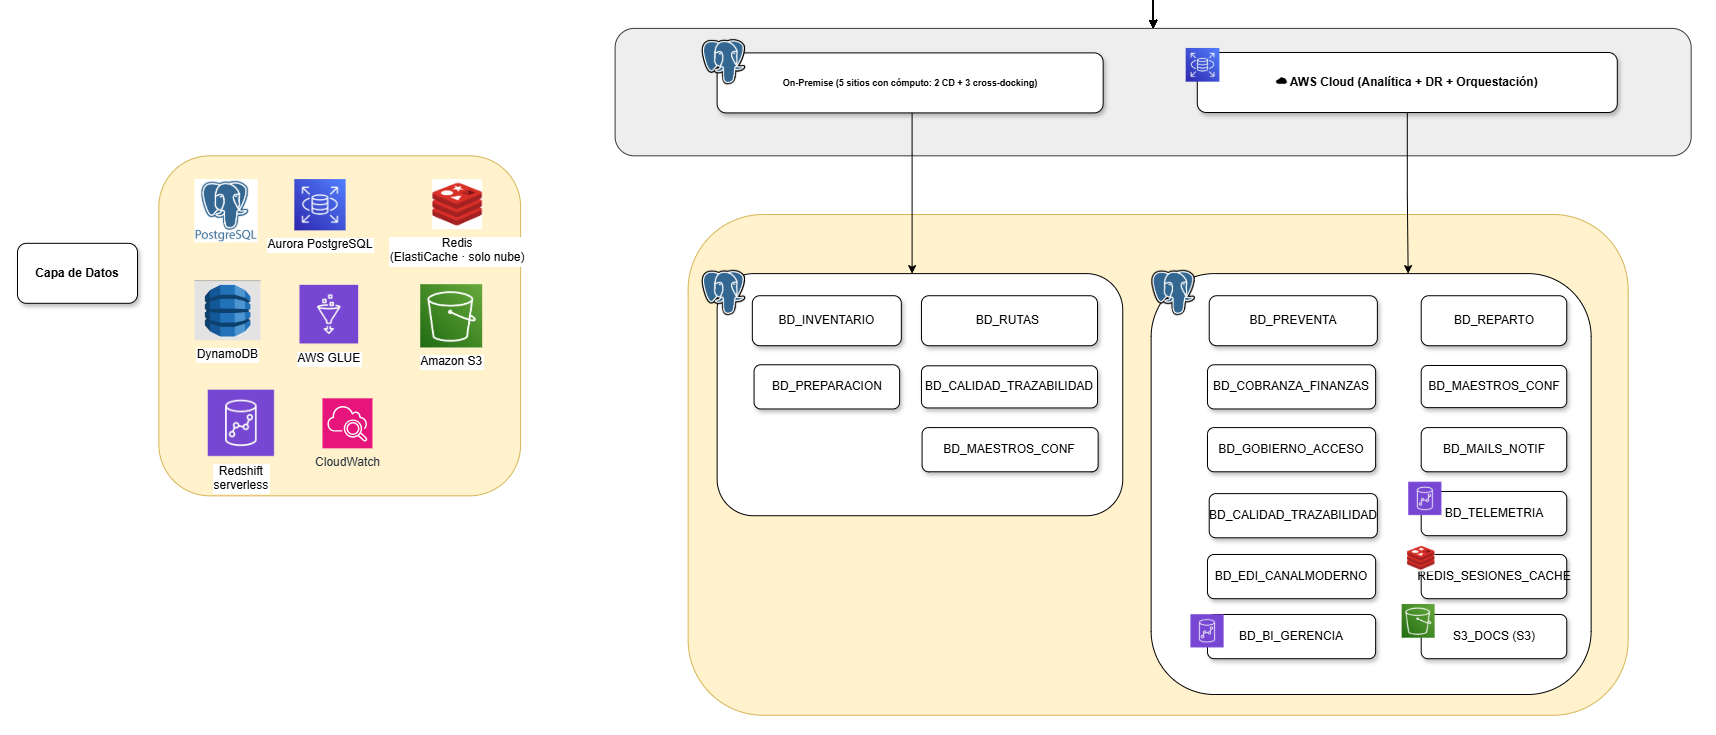
\includegraphics[width=0.98\linewidth,height=0.60\textheight,keepaspectratio]{Diagramas/arquitectura_logica_actual/capas_recortes/ARQL-26_Recorte_Datos.png}
  \captionof{figure}{Datos: propiedad y persistencia híbrida}
  \label{fig:arql-capa-6}
  \par\smallskip
  {\raggedright\footnotesize Fuente: recorte por capa del diagrama general aportado por Tomás Pérez; LafroX.\par}
  \end{minipage}
\end{center}

El sitio conserva la autoridad de bodega y el dispositivo mantiene sus capturas hasta recibir confirmación durable. Los servicios centrales separan transacciones, caché, documentos y analítica; ninguna consulta de BI debe competir con el despacho.


La capa de datos distingue quién conserva la información operativa, quién la consolida y quién la consulta para análisis. Esta separación permite que la bodega siga trabajando sin enlace externo y que las consultas gerenciales no compitan con el despacho. Los dominios de información asumen las siguientes responsabilidades:

En la operación local:
\begin{itemize}
  \item \textbf{CD Talca:} PostgreSQL 16 con PostGIS como maestro de bodega para recepción, preparación y despacho, con autonomía mínima de 24 horas.
  \item \textbf{CD Concepción:} PostgreSQL y WMS de alcance reducido (\texttt{wms\_only}), capaz de sostener 24 horas de operación local sin depender de Talca.
  \item \textbf{Cross-docking de Curicó, Chillán y Los Ángeles:} mini-WMS para registrar recepción, desconsolidación y despacho. El detalle se sincroniza con Talca y los eventos críticos se publican en SQS FIFO cuando existe conexión. Las tres horas indicadas en el caso son una ventana operativa, no una excepción a RT-03.10: el diseño lógico exige al menos 24 horas de continuidad local degradada, cuya suficiencia deberá demostrarse mediante pruebas.
\end{itemize}

En los servicios centrales, PostgreSQL conserva las transacciones de preventa, reparto y canal moderno; el flujo de telemetría ingresa en DynamoDB y se consolida para análisis en S3 y Redshift mediante Glue; Redis acelera lecturas autorizadas de stock, precios y sesiones; S3 conserva documentos y evidencias. La función de cada almacén, y no su ubicación física, determina qué módulo puede escribir en él. La topología de replicación y recuperación se especifica en 4.2.

No se incorpora Redis local. Al iniciar el turno con conexión, la aplicación solicita a las APIs una copia de stock, precios y demás datos autorizados; los servicios la obtienen de sus almacenes, incluido ElastiCache. El dispositivo conserva esa copia cifrada en SQLite/Room y consulta allí mientras está desconectado. Al reconectar, reconcilia primero las escrituras pendientes y actualiza los datos de lectura. Reemplazar la copia de lectura nunca debe borrar pedidos, cobros ni evidencias aún no confirmados por el servidor.

La vigencia de los datos de lectura es independiente de la identidad. Las credenciales de turno duran 8 horas en bodega y 14 horas en terreno; la caché local de identidad es de solo lectura y tiene TTL de 24 horas en VM-05 (Talca), VM-C03 (Concepción) y E-01 de cada cross-docking. Una copia reciente de precios no renueva la sesión y una sesión válida no convierte el stock descargado en una reserva confirmada. El relevo de turno sin IdP lo habilita el verificador local del mismo nodo, conforme a la capa de seguridad de este apartado.

La separación transaccional/analítica es estricta: la analítica no lee del transaccional para evitar degradar la ventana crítica de despacho. Las latencias comprometidas son: operación del día $\leq$ 5 minutos, cierre comercial $\leq$ 2 horas, gestión $\leq$ 4 horas.

Cada evento conserva identidad, estado y resultado hasta recibir confirmación durable. DMS replica el WMS de Talca hacia un esquema de lectura; no escribe en las tablas de negocio centrales. Los consumidores de eventos actualizan estas últimas con deduplicación transaccional por sitio y UUID. Concepción y los cross-docking sincronizan sus eventos sin presumir un flujo DMS propio. Durante un corte cada sitio retiene sus cambios dentro de una capacidad comprobada para 24 horas. Esta retención no acredita el RPO ante destrucción del origen: se exige protección durable fuera de su dominio de falla y la prueba del Anexo 4.1-M. El esquema 3-2-1-1-0, los medios de respaldo y la restauración se desarrollan en 4.2.

\subsubsection{Capa de seguridad transversal (Capa 7)}

La Figura~\ref{fig:arql-capa-7} presenta las responsabilidades de esta capa.

\begin{center}
  \begin{minipage}{\linewidth}\centering
  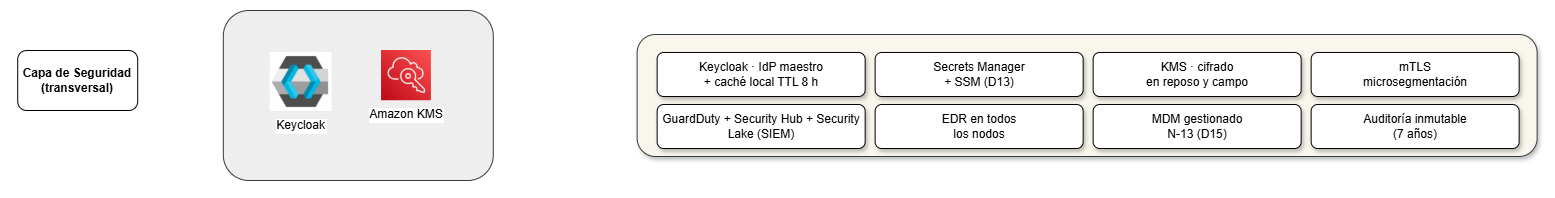
\includegraphics[width=0.98\linewidth,height=0.60\textheight,keepaspectratio]{Diagramas/arquitectura_logica_actual/capas_recortes/ARQL-27_Recorte_Seguridad.png}
  \captionof{figure}{Seguridad: identidad y autorización transversal}
  \label{fig:arql-capa-7}
  \par\smallskip
  {\raggedright\footnotesize Fuente: recorte por capa del diagrama general aportado por Tomás Pérez; LafroX.\par}
  \end{minipage}
\end{center}

Keycloak emite la identidad y cada módulo decide la autorización sobre su recurso. Sin enlace, el verificador usa permisos de turno previamente firmados; el cifrado y la auditoría protegen los datos y decisiones a lo largo de todas las capas.


La seguridad atraviesa las ocho capas. Su unidad de decisión no es la red desde la que llega una solicitud, sino el sujeto, el recurso, la acción y el contexto del turno. Keycloak conserva la autoridad de identidad; el servicio dueño del recurso conserva la decisión de autorización. Esta separación evita que un token válido permita, por sí solo, liberar una carga, consultar crédito o modificar una regla de calidad (PUCV, 2026b, caps.~11--12, pp.~23--26; RT-11.01 y RT-12.05; National Institute of Standards and Technology [NIST], 2020).

\paragraph{Límites de confianza y capa expuesta.}
La Figura~\ref{fig:arql-1} distingue personas, dispositivos, sitio, servicios centrales y terceros. CloudFront protege los portales externos y sus APIs; el origen de esas APIs rechaza el acceso público directo. Las consolas internas usan acceso verificado por identidad y postura del dispositivo hacia servicios privados. OpenAS2 expone un canal B2B distinto, limitado a contrapartes registradas y con validación criptográfica y MDN; no es una API pública de negocio. Los almacenes de datos no son superficies públicas. El inventario de dominios, puertos y rutas de 4.2 debe representar las tres superficies por separado (RT-11.07 y RT-11.13).

API Gateway verifica la identidad, el alcance, las cuotas, los límites de tasa, el esquema y la carga útil antes de entregar una solicitud; M1--M12 repiten la autorización de negocio sobre el recurso concreto. Los puntos públicos incorporan detección de bots y reto progresivo sin bloquear a una persona legítima. La comunicación entre servicios se autentica mutuamente y se cifra; un evento asíncrono también conserva productor, destinatario, versión, identificador y permisos necesarios. Así se aplica el mismo límite de confianza a REST y a mensajería (RT-11.11--11.12).

La política lógica prohíbe el ingreso público directo a los sitios. Las excepciones de integración a través de un túnel privado no son exposición a internet: se autorizan de forma nominativa, por origen, destino y propósito, y se registran. Su número, sentido de inicio de conexión y reglas de red deben quedar inequívocos en 4.2; una excepción no amplía el permiso de los módulos para escribir directamente en el ERP.

\paragraph{Identidad, autorización y sesiones.}
La identidad central utiliza OIDC, SSO y MFA. El rol se complementa con atributos de instalación, turno, ruta, dispositivo y empresa transportista. El proveedor solo consulta sus órdenes; el transportista administra sus conductores y rutas asignadas; el conductor actúa sobre su entrega y rendición; Calidad decide sobre un lote bloqueado; y Tesorería aprueba la conciliación, sin que quien registró el cobro pueda aprobar su propia diferencia. Los administradores elevan privilegios por tiempo limitado, con aprobación y registro de sesión. El alta, cambio de rol y baja quedan vinculados al ciclo de vida laboral o contractual; las personas externas disponen de registro, verificación y recuperación de acceso sin requerir correo corporativo (RT-12.01--12.06 y RT-12.09--12.12).

En las APIs Laravel, un guard OIDC comprueba firma con las claves publicadas por Keycloak, emisor, audiencia, vencimiento y alcance. Las políticas del módulo dueño verifican además recurso, turno y atributos; se prueban tanto rutas HTTP como trabajos asíncronos para que una cola no eluda la autorización. El acceso local usa exclusivamente el verificador de manifiestos descrito abajo. Laravel no emite otra identidad de usuario mediante Sanctum o Passport: Keycloak sigue siendo el único IdP y la administración de personas se realiza en el portal Angular autorizado.

En conexión, el token de acceso dura como máximo 30 minutos; la inactividad cierra la sesión administrativa a los 15 minutos y las demás a los 30. La credencial de refresco es rotatoria, se invalida ante baja o sospecha de compromiso y no supera 24 horas para acceso ordinario ni 8 horas para privilegios. El cierre de sesión se propaga a los servicios conectados y se impide la concurrencia no autorizada para cuentas compartibles por riesgo. Ninguna credencial se transporta en la URL. Estas duraciones no renuevan ni alargan una autorización offline; responden a los controles de RT-12.07--12.08.

La credencial de turno dura hasta 8 horas en bodega y hasta 14 horas en terreno. Mientras existe enlace, Keycloak renueva al menos cada hora un manifiesto firmado con los turnos y permisos preinscritos para una ventana de 26 horas; así, incluso si el corte comienza justo antes de la renovación siguiente, quedan al menos 25 horas de verificación local. La caché de identidad, de solo lectura y TTL de 24 horas, conserva datos recibidos en VM-05 (Talca), VM-C03 (Concepción) y E-01 de cada cross-docking, pero no emite sesiones. Al relevarse un turno sin enlace, el verificador del mismo nodo comprueba la firma y vigencia del manifiesto y un segundo factor local: el PIN personal sobre el terminal enrolado por MDM; limita el acceso a M1, M2, M5 y a las acciones autorizadas de M9, bloquea intentos repetidos y registra cada decisión. El dispositivo compartido identifica el contexto, pero no sustituye la identidad personal del operario. Los detalles de claves y alojamiento pertenecen a 4.2 (ADR-06).

La revocación es inmediata en los servicios conectados. Durante una desconexión no se promete revocación remota instantánea: el permiso local expira al terminar su turno, no se amplía sin enlace y la incidencia se marca para revisar operaciones al reconectar. Una baja conocida localmente bloquea de inmediato la credencial en ese sitio; el verificador sincroniza las revocaciones y auditorías al restablecerse el enlace. Se ensayan dos relevos dentro de 24 horas, vencimiento, pérdida de dispositivo y recuperación del enlace. La cuenta de emergencia exige doble autorización, alcance acotado, custodia fuera de banda, registro y rotación posterior; no reemplaza la autenticación ordinaria de todos los operarios (RT-03.10 y RT-12.13).

\paragraph{Clasificación, cifrado y custodia.}
La Tabla~\ref{tab:seguridad-clasificacion} resume cómo cambia el control según el dato. La clasificación se aplica al evento, su copia local, las APIs y las exportaciones, no solo a la base de datos central.

\begin{tablalafrox}{Clasificación lógica y protección de la información}{tab:seguridad-clasificacion}{F{0.17} F{0.29} F{0.28} Y}{\cab{Nivel} & \cab{Ejemplo del caso} & \cab{Regla de acceso} & \cab{Protección adicional}}
Restringido & Credenciales, claves y factores. & Solo custodios nominados. & Claves separadas y auditoría. \\
Confidencial & Crédito, conducta de pago, geolocalización y POD. & Rol, finalidad y registro de consulta. & Cifrado por campo sensible. \\
Interno & Pedidos, movimientos y telemetría operativa. & Módulo dueño y perfiles autorizados. & Cifrado y trazabilidad. \\
Público & Catálogo sin precios. & Lectura anónima controlada. & Integridad y protección antiabuso. \\
\end{tablalafrox}

{\footnotesize Fuente: elaboración propia de LafroX a partir de Bases Técnicas Transversales, RT-11.03/09/10, y Caso 02, capítulo 15.\par}

La categoría confidencial exige separar quién puede usar el dato de quién administra su almacenamiento: el acceso a la base no revela por sí solo comportamiento de pago ni geolocalización. Todo dato en reposo se cifra; los campos sensibles del caso reciben además cifrado por campo. En tránsito se exige TLS 1.3 para las interfaces compatibles, se prohíben TLS 1.0 y 1.1, se automatiza la gestión de certificados y se emplea mTLS entre servicios. La custodia y rotación de claves mantienen separación de funciones. El PAN de tarjetas no se almacena; se usa la tokenización de la pasarela. El RUT requiere una técnica de seudonimización con acceso a la clave separado y una finalidad documentada, sin confundir cifrado reversible con anonimización. La geolocalización de personas conserva la retención de 12 meses del caso y un registro de consultas; su transferencia fuera de Chile depende de la evaluación y aprobación aplicables, no de la existencia técnica de una réplica (PUCV, 2026a, cap.~15, pp.~26--30; PUCV, 2026b, cap.~11, pp.~23--24; RT-11.08--11.10 y RT-16.09).

\paragraph{Amenazas, controles y evidencia.}
El modelado STRIDE toma cada módulo y cada integración externa como unidad de revisión, identifica su límite de confianza, abuso posible, mitigación, responsable y prueba. Para M3, el abuso es reutilizar una credencial o reenviar un pedido: se comprueban enrolamiento, vigencia e idempotencia. Para M5, la elevación indebida de privilegios no debe liberar una carga bloqueada por M9: se prueba la separación de autorizaciones. Para M11 y la ACL, un mensaje EDI repetido o manipulado se rechaza o aísla sin escribir dos veces en el ERP. El Anexo 4.1-Q registra las amenazas por módulo y frontera; el Anexo 4.1-R vincula controles ISO/IEC 27001/27002 con responsable y prueba. Son especificaciones de aceptación, no resultados de ensayos ni certificación (ISO, 2022b, 2022c) (RT-11.02 y RT-11.05).

Cada decisión de acceso y cada acción crítica conserva sujeto, empresa si aplica, recurso, operación, resultado, hora, identificador de transacción y regla aplicada. Los eventos de seguridad se envían a una bitácora inalterable y al SIEM; durante un corte se conservan localmente y se remiten con el mismo identificador al reconectar. Las reglas de detección incluyen acceso privilegiado fuera de turno, intentos reiterados de uso de una credencial de conductor revocada, consulta masiva de datos comerciales, alteración de evidencia de temperatura y desvío anómalo de mensajes EDI. Los registros técnicos en CloudWatch se conservan 12 meses en línea y 24 meses adicionales en archivo; los registros de seguridad y auditoría se conservan 7 años bajo Object Lock. La retención de documentos tributarios y POD se gobierna separadamente por su dominio de datos. La plataforma y el SOC que operan estos controles se describen en 4.2 y en el capítulo de servicios (RT-11.14--11.19).

La aceptación de esta vista requiere una prueba de acceso denegado por rol y atributo, una de cifrado de campo con lectura administrativa sin texto claro, una de continuidad y relevo offline, una de revocación al reconectar y una de correlación de un evento de negocio con su alerta de seguridad. Se distinguen dos objetivos de disponibilidad: 99,95 \% mensual para la infraestructura del recinto y al menos 99,9 \% mensual para el servicio de negocio de extremo a extremo. Ninguno elimina la exigencia de continuidad durante el despacho de 05:30 a 07:00.

\subsubsection{Capa de observabilidad transversal (Capa 8)}

La Figura~\ref{fig:arql-capa-8} presenta las responsabilidades de esta capa.

\begin{center}
  \begin{minipage}{\linewidth}\centering
  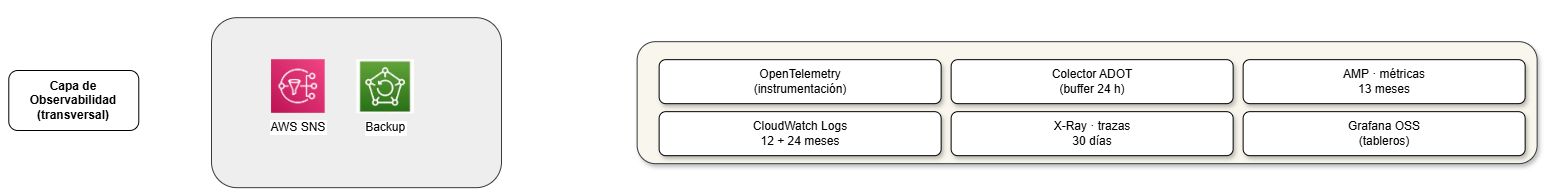
\includegraphics[width=0.98\linewidth,height=0.60\textheight,keepaspectratio]{Diagramas/arquitectura_logica_actual/capas_recortes/ARQL-28_Recorte_Observabilidad.png}
  \captionof{figure}{Observabilidad: correlación de nube y sitios}
  \label{fig:arql-capa-8}
  \par\smallskip
  {\raggedright\footnotesize Fuente: recorte por capa del diagrama general aportado por Tomás Pérez; LafroX.\par}
  \end{minipage}
\end{center}

La correlación permite seguir una operación entre APIs, módulos y consumidores. Durante el corte, el sitio conserva telemetría y mantiene sus alarmas; CloudWatch reúne registros, métricas y trazas para los tableros y la atención de incidentes.


La observabilidad debe ayudar al equipo a responder preguntas operativas: qué pedido quedó pendiente, dónde se interrumpió una integración y qué entregas pueden verse afectadas. Para ello reúne métricas, registros y trazas de nube y sitios locales en una misma plataforma (RT-03.16 y Art. 16.4).

La instrumentación utiliza OpenTelemetry para PHP/Laravel y las aplicaciones Kotlin, junto con los registros y métricas disponibles de API Gateway, RabbitMQ, SQS y Greengrass. El identificador \texttt{transaction\_id} acompaña las solicitudes y los mensajes; los trabajadores extraen el contexto de traza del sobre de evento para correlacionar la operación de negocio, incluidos los procesos asíncronos.

En on-premise, los colectores ADOT, con buffer en disco de 24 horas, recolectan la telemetría local y la exportan a la plataforma única en Amazon CloudWatch: Logs conserva los registros técnicos 12 meses en línea y 24 meses en archivo; Metrics conserva las métricas 13 meses; las trazas y los tableros operacionales también se alojan en CloudWatch (ADR-14).

Los tableros se estructuran en tres niveles: operacional (para el equipo de TI y SRE), gerencial (para la gerencia y jefes) y del mandante (para Puelche, solo lectura con auditoría de consultas, conforme a RT-14.02). Las alertas se formulan por síntomas de negocio, no por causas técnicas, con ventanas de evaluación para evitar falsos positivos y escalamiento por criticidad.

Durante un corte de enlace, el sitio no depende de los tableros centralizados para despachar. Las alarmas locales continúan y los colectores retienen la telemetría para enviarla al restablecer la conexión. La capacidad del buffer de 24 horas debe comprobarse con la carga de diseño; no se presume conservación ilimitada. La retención de métricas, registros técnicos y trazas no sustituye la política de auditoría de negocio exigida por RT-16.10.

